\documentclass[a4paper, 12pt]{report}

\usepackage[french]{babel}
\usepackage[T1]{fontenc}
\usepackage[]{geometry}
\usepackage{blindtext}
\geometry{
 a4paper,
 total={170mm,250mm},
 left=20mm,
 top=30mm,
 }
\addtolength{\textwidth}{1.0cm}
\usepackage{newtxtext, newtxmath}
\usepackage{graphicx}
\usepackage{caption}
\usepackage{subcaption}
\usepackage{xcolor}
\definecolor{RoyalRed}{RGB}{255,165,0}

\usepackage{minted}
\setminted[dart]{
  frame=lines,
        framesep=2mm,
        baselinestretch=1.2,
        fontsize=\footnotesize,
        linenos,
}

\usepackage{listings}
\usepackage{parcolumns}

\usepackage{tikz}
\tikzstyle{start} = [rectangle, rounded corners, minimum width=3cm, minimum height=1cm,text centered, draw=RoyalRed]

\usepackage{fancyhdr}
\pagestyle{fancy}

\pagestyle{fancy}
\fancyhf{}
\rhead{\color{RoyalRed} CHAPITRE \thechapter}
\lhead{\rightmark}
\rfoot{\thepage}



\usepackage{titlesec}
\titleformat{\chapter}[display]
{\vspace*{-5cm}\normalsize \huge  \color{black}}%
  {\flushright\normalsize \color{RoyalRed}%
   \MakeUppercase{\chaptertitlename}\hspace{1ex}%
   {\fontsize{60}{60}\selectfont\thechapter}}%
  {1 pt}%
  {\bfseries\huge}%
  [\vspace*{-1.0cm}]%

\usepackage{parskip}%
\setlength{\parindent}{0pt}
\setlength{\headheight}{15pt}
% \setlength{\parskip}{\baselineskip}

\begin{document}

\begin{titlepage}
    \begin{center}
        \vspace*{1cm}

        \Huge
        \textsf{\textbf{L'application Crazy Wolf}}
 
        \vspace{0.5cm}
        \LARGE
        \texttt{Application smartphone pour la gestion des horaires
        et des services du personel du restaurant Crazy Wolf}
             
        \vspace{1.5cm}
        \large
        \underline{\texttt{TRAVAIL DE BACHELOR}}

        \vspace{2.0cm}
        \Large
        DANIEL SANZ \\
        \large
        Décembre 2020
             
        \vspace{2.0cm}
        \textbf{Supérvisé par:}\\
        Prof. Dr. Jacques Pasquier\\
        et\\
        Pascal Gremaud\\
        Software Engineering Group
        \vfill
        \hrulefill

        \begin{minipage}[c]{0.2\textwidth}
            \centering
            
\includegraphics{logos/unifr_logo.png}   
        \end{minipage}
        \begin{minipage}[c]{0.4\textwidth}
            \centering
            \normalsize
            Groupe Génie Logiciel\\
            Département d'informatique\\
            Université de Fribourg (Suisse)
        \end{minipage}
        \begin{minipage}[c]{0.3\textwidth}
            \centering

            
\includegraphics[scale=0.25]{logos/softeng.png}   
        \end{minipage}

             
    \end{center}
 \end{titlepage}

\tableofcontents

\chapter[Introduction]{Introduction}
\cite{einstein}
La bonne gestion des ressources dans une entreprise est inaliénable à son bon fonctionnement. Le personnel et son horaire de travail l'est, par extension, également. 

Un petit restaurant aurait du mal à investir dans un \textbf{ERP}\footnote{Entreprise Resources Planning} pour gérer l'attribution des horaires de son personnel. De plus, ceux-ci sont conçu pour une certaine stabilité et non pas pour des changements très fréquents.

En collaboration avec le restaurant du Crazy Wolf, à Fribourg, j'ai développé une application pour gérer les horaires et les échanges de services du personnel.

\section[Motivations et objectifs]{Motivation et Objectifs}

\subsection*{Motivation}
J'ai travaillé un an dans le restaurant du Crazy Wolf.

En ce qui concerne les serveurs, il y en a beaucoup. Environ une quinzaine. Pendant cette année de travail j'ai constaté que les serveurs, étant majoritairement étudiants, avaient, pour la plupart, de petits pourcentages d'occupation. Un ou deux services par semaine. Par service en entend la tranche horaire de travail de midi ou du soir. 
De par la jeunesse du personnel et des occupations annexes que les serveurs ou serveuses ont, les échanges sont très fréquents. 

Actuellement le restaurant du Crazy Wolf utilise une messagerie instantanée pour gérer la distribution d'horaires, les échanges entre les serveurs, les imprévus, \dots Et ce, avec les inconvénients qui s'imposent: les demandes de remplacements se perdent dans l'historique de conversation, du personnel oublie de se présenter, le même message et répété plusieurs fois, entre autres aléas.



Ainsi, l'idée d'une gestion centralisée de l'horaire et des échanges de services m'est venu. En discutant avec plusieurs membres du personnel et avec les patrons, ils ont confirmé que cette idée répondait à une problématique réelle. 

\subsection*{Objectifs}

Créer une application disponible sur Android et IOS pour la gestion des horaires et des échanges. L'objectif est mesurable. En effet, si la messagerie instantanée n'est plus ou très peu utilisé alors la création d'une application se justifie.

\newpage

\section[Structure du rapport]{Structure du rapport}

\subsection*{Chapitre I: Introduction}
L'introduction est le discours préliminaire de ce rapport.

\subsection*{Chapitre II: Aspects métier}
Dans ce chapitre se trouve l'analyse de la problématique d'un point de vue métier. C'est-à-dire, les conditions d'utilisation, le type d'utilisateurs, définitions claires d'utilisation. Précisions sur le résultat recherché.

\subsection*{Chapitre III: Présentation de l'application}
Dans ce chapitre l'application est présentée. Son mode de fonctionnement ainsi que des captures d'écran pour décrire plusieurs scénarios d'utilisations possibles.

\subsection*{Chapitre IV: Éléments de programmation}
Dans ce chapitre se situe la partie technique en lien avec l'implémentation. On y retrouve la description du framework utilisé ainsi que les points clefs du développement, au travers d'extraits du code source commentés.

% \subsection*{Chapitre V: Coordination avec le client}
% L'application développée s'est faite en accord avec le restaurant du Crazy Wolf. Dans ce chapitre seront résumés les contacts avec ce dernier ainsi que nos différents échange ou encore les fonctionnalités demandées.

\subsection*{Chapitre V: Conclusion}
Dans ce chapitre seront discutés les résultats du projet. De plus, j'y fais part de mon point de vue personnel.

% \section[Table des symboles]{Conventions d'écriture}



\chapter[Domaine métier]{Domaine métier}
Dans le restaurant Crazy Wolf et dans la restauration en général, les employés sont susceptibles de ne pas travailler tous les jours ou de ne pas travailler toute la journée mais seulement certains "services".

Un service est une tranche horaire qui correspond aux heures pendant lesquelles le restaurant offre un service de restauration. Dans le cas concret du Crazy Wolf, il y a deux services: midi et soir. Qui englobent les heures de travail de 9h00 à 15h00 et de 17h00 à 23h00 respectivement. Dans ces tranches horaires sont incluses les heures nécessaires à la disposition du restaurant et d'autres préparations nécessaires avant l'arrivée de clients.

De plus, dans la restauration et surtout en ce qui concerne les serveurs, il est commun d'y trouver trois types d'acteurs avec différents statuts: 
\smallskip
\begin{itemize}
    \item serveur$\cdot$euses
    \item manager 
    \item patrons
\end{itemize}
\smallskip
La gestion, visualisation et organisation des services parmi ces trois acteurs est un élément vital pour un restaurant.

\section[Analyse]{Analyse}
D'après mon observation, la planification de l'horaire de travail des serveurs à un moment donné n'est pas invariante par rapport au temps. En d'autres termes, entre le moment où l'attribution de services aux serveurs est faite et le moment où un serveur y travaille effectivement il peut y avoir de grandes variations. J'ai constaté essentiellement trois facteurs susceptibles de perturber la planification initial:
\smallskip
\begin{itemize}
    \item le désistement d'un$\cdot$e serveur$\cdot$euses
    \item les échanges
    \item la demande de renfort de la part du manager ou d'un patron.
\end{itemize}
\smallskip
Le premier peut être dû à diverses raisons: maladie, imprévu... De plus comme dans le Crazy Wolf, la majorité des serveur$\cdot$euses sont étudiant$\cdot$es les révisions et examens sont fréquemment cause de désistement.

Le deuxième est le fruit d'un mutuel accord entre deux serveurs pour échanger leurs services.

Le troisième est le fruit de l'analyse d’affluence  des clients de la manager en accord avec les patrons. En effet, s'ils constatent que subitement l'afluence des clients augmente le jeudi soir et qu'il y a de fortes chances pour que ce soit aussi le cas le vendredi soir, il sera nécessaire de demander un ou des serveurs supplémentaires. 

Les raisons de cette affluence augmentée peuvent être très diverses. Les conditions météo par exemple. Plus de gens vont au Crazy Wolf quand il pleut, ou en hiver. Ou encore des manifestations comme carnaval ou le marathon.

Dans le jargon propre au Crazy Wolf, ces serveurs supplémentaires sont appelés "doubleurs".

Ainsi, la gestion des horaires est dynamique et non statique.
\newpage
\section[Problématique]{Définition de la problématique}
Actuellement, le Crazy Wolf utilise un groupe, contenant tout le personnel, d'une messagerie instantanée pour communiquer. Dans ce groupe sont traités toute sorte d'aspects. Depuis des félicitations d'anniversaires, jusqu'à l'envoi des horaires mensuels sous forme PDF en passant par des discutions d'échanges, de remplacements, de renforts ou encore sur des discutions relatives aux normes sanitaires dues à la pandémie du COVID-19. 

Ainsi, lorsque la manager demande un renfort pour dans deux semaines et que personne ne se porte volontaire immédiatement, il y a de grandes chances que le message soit répété plusieurs fois.

Il est donc nécessaire de disposer d'une plateforme dynamique, standardisée, centralisée et intuitive dédiée exclusivement à la gestion des horaires. 

Cette plateforme doit être accessible en tout temps depuis internet. Une application fonctionnant sur les deux principaux systèmes d'exploitation mobiles répond bien à ce besoin.

En somme, cette application doit fournir les fonctionnalités suivantes:

\subsection*{Login}
L'application doit permettre aux utilisateurs de s'authentifier pour accéder à l'ensemble des fonctionnalités.

\begin{figure}[!h]
    \begin{center}
        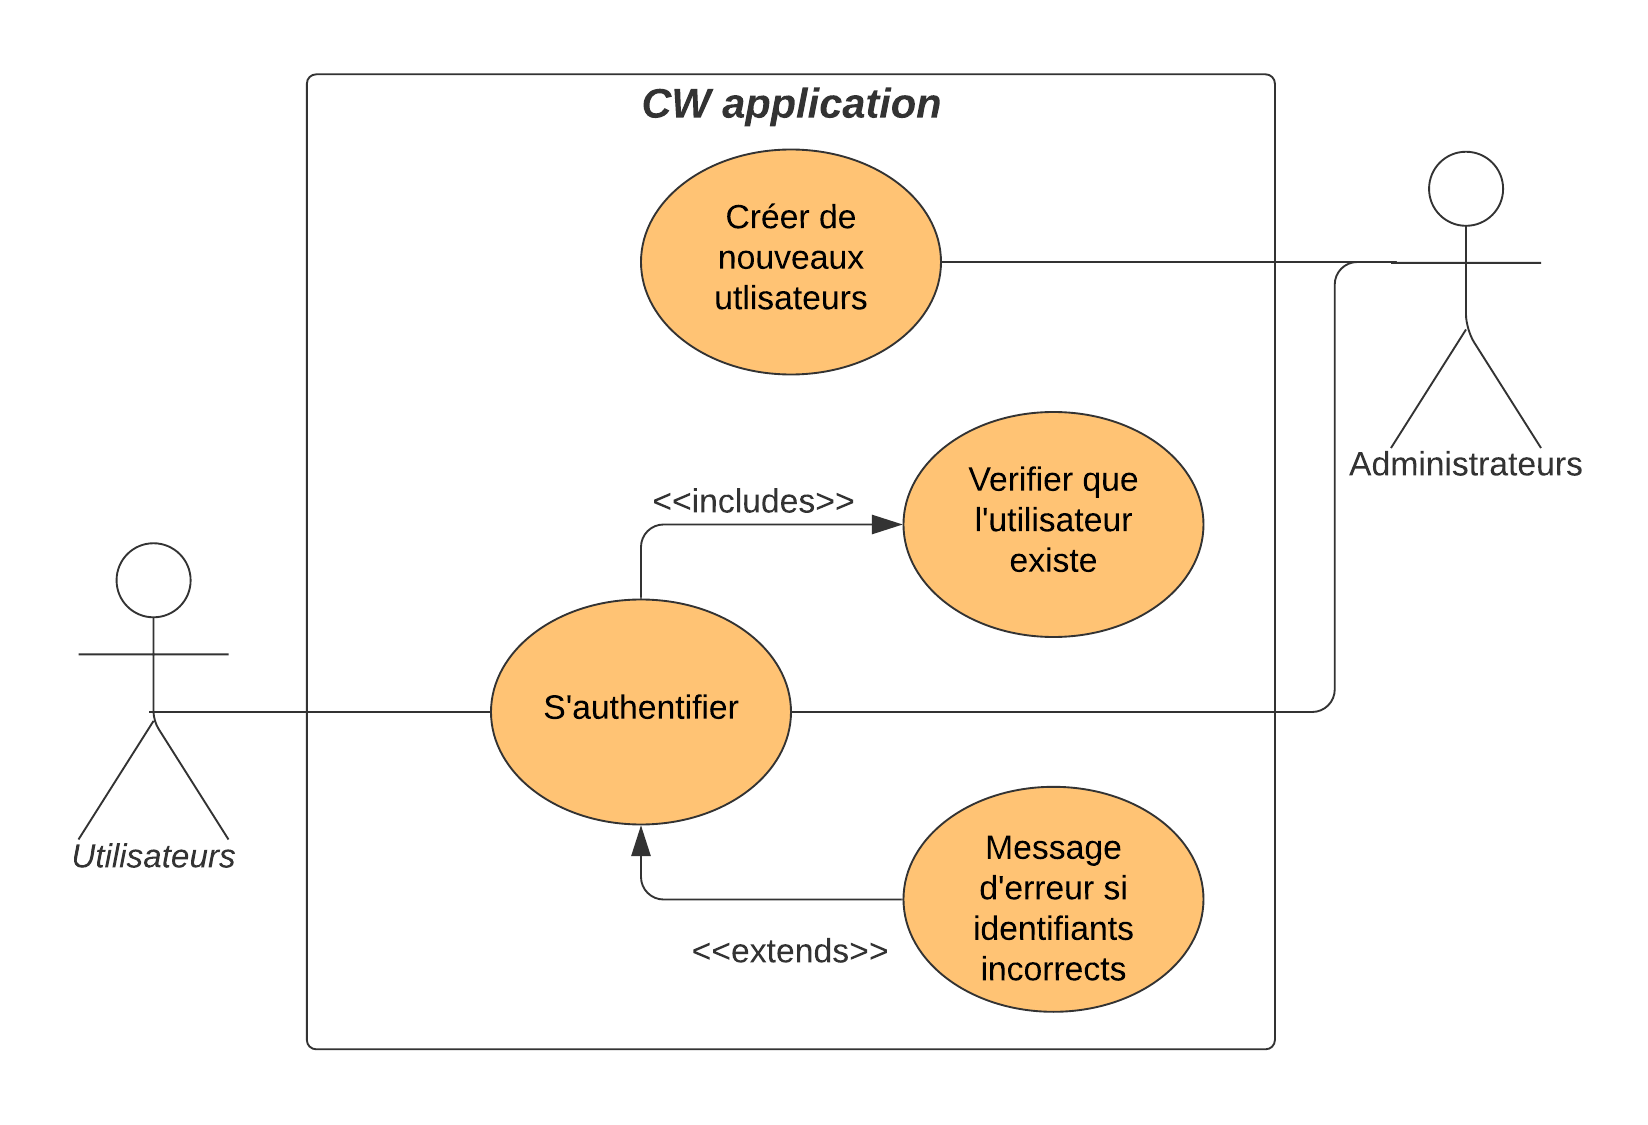
\includegraphics[width= 0.8\textwidth]{uses cases/logginUC.png}
    \end{center}
    \caption{use case: login}
\end{figure}

Pour que l'authentification soit validée, l'utilisateur doit posséder des identifiants qu'un administrateur à créer précédemment. Attention, administrateur doit aussi s'authentifier pour pouvoir créer de nouveaux utilisateurs.

De plus, les utilisateurs doivent être informés si leur saisie est incorrecte.

\subsection*{Visualiser les services}
L'application doit permettre à tous les utilisateurs de consulter rapidement et facilement les services dans lesquels ils travaillent. De plus, ils doivent également pouvoir voir les services dans lesquels les autres utilisateurs travaillent. En effet, il n'y a là aucune information confidentielle.

\begin{figure}[!h]
    \begin{center}
        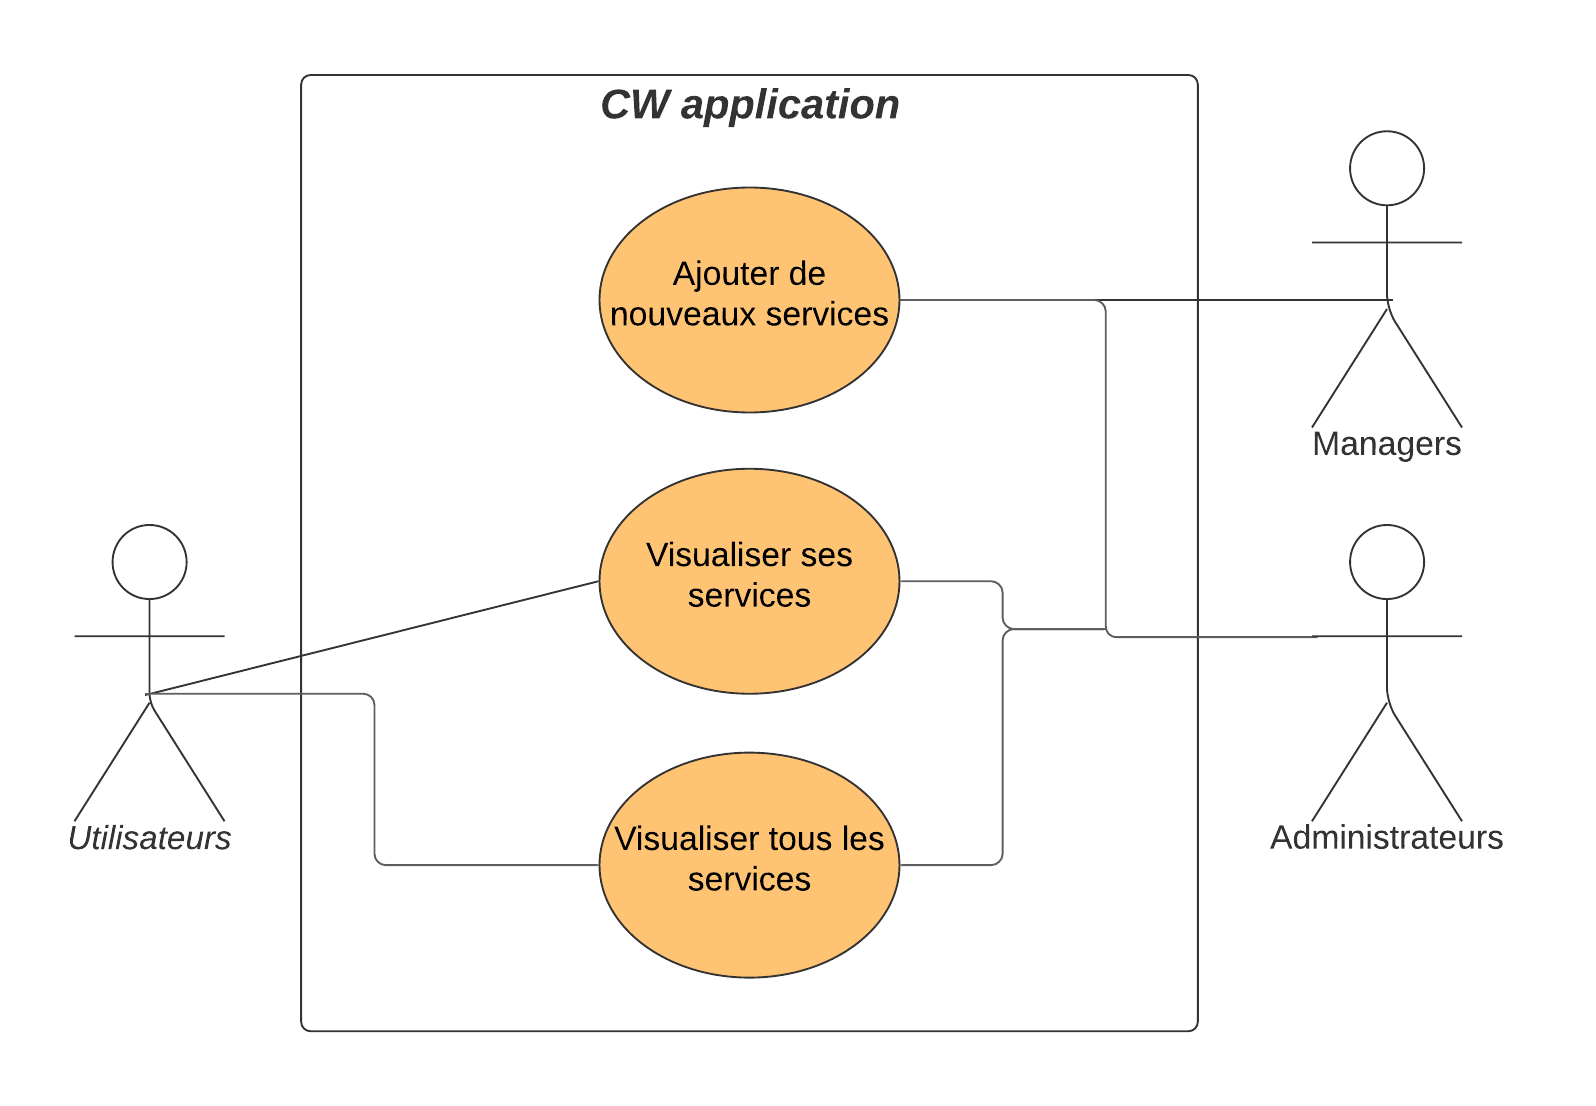
\includegraphics[width= 0.8\textwidth]{uses cases/visualiser services.png}
    \end{center}
    \caption{use case: visualisation des services}
\end{figure}

Afin de pouvoir visualiser des services, il est nécessaire que préalablement, un manager ou un administrateur en ait ajouté dans le système. De plus, le niveau de permission n'exclut pas la possibilité qu'un manager ou administrateur aient des services dans lesquels ils travaillent. Ainsi, ils doivent également pouvoir les visualiser.

\newpage

\subsection*{Mise en bourse}

La mise en bourse d'un service est la fonctionnalité principale de l'application. L'application doit permettre à un$\cdot$e serveur$\cdot$euse de pouvoir mettre un service, où il ou elle ne peut pas travailler, en bourse afin que d'autres utilisateurs de l'application puissent le ou la remplacer.
\begin{figure}[!h]
    \begin{center}
        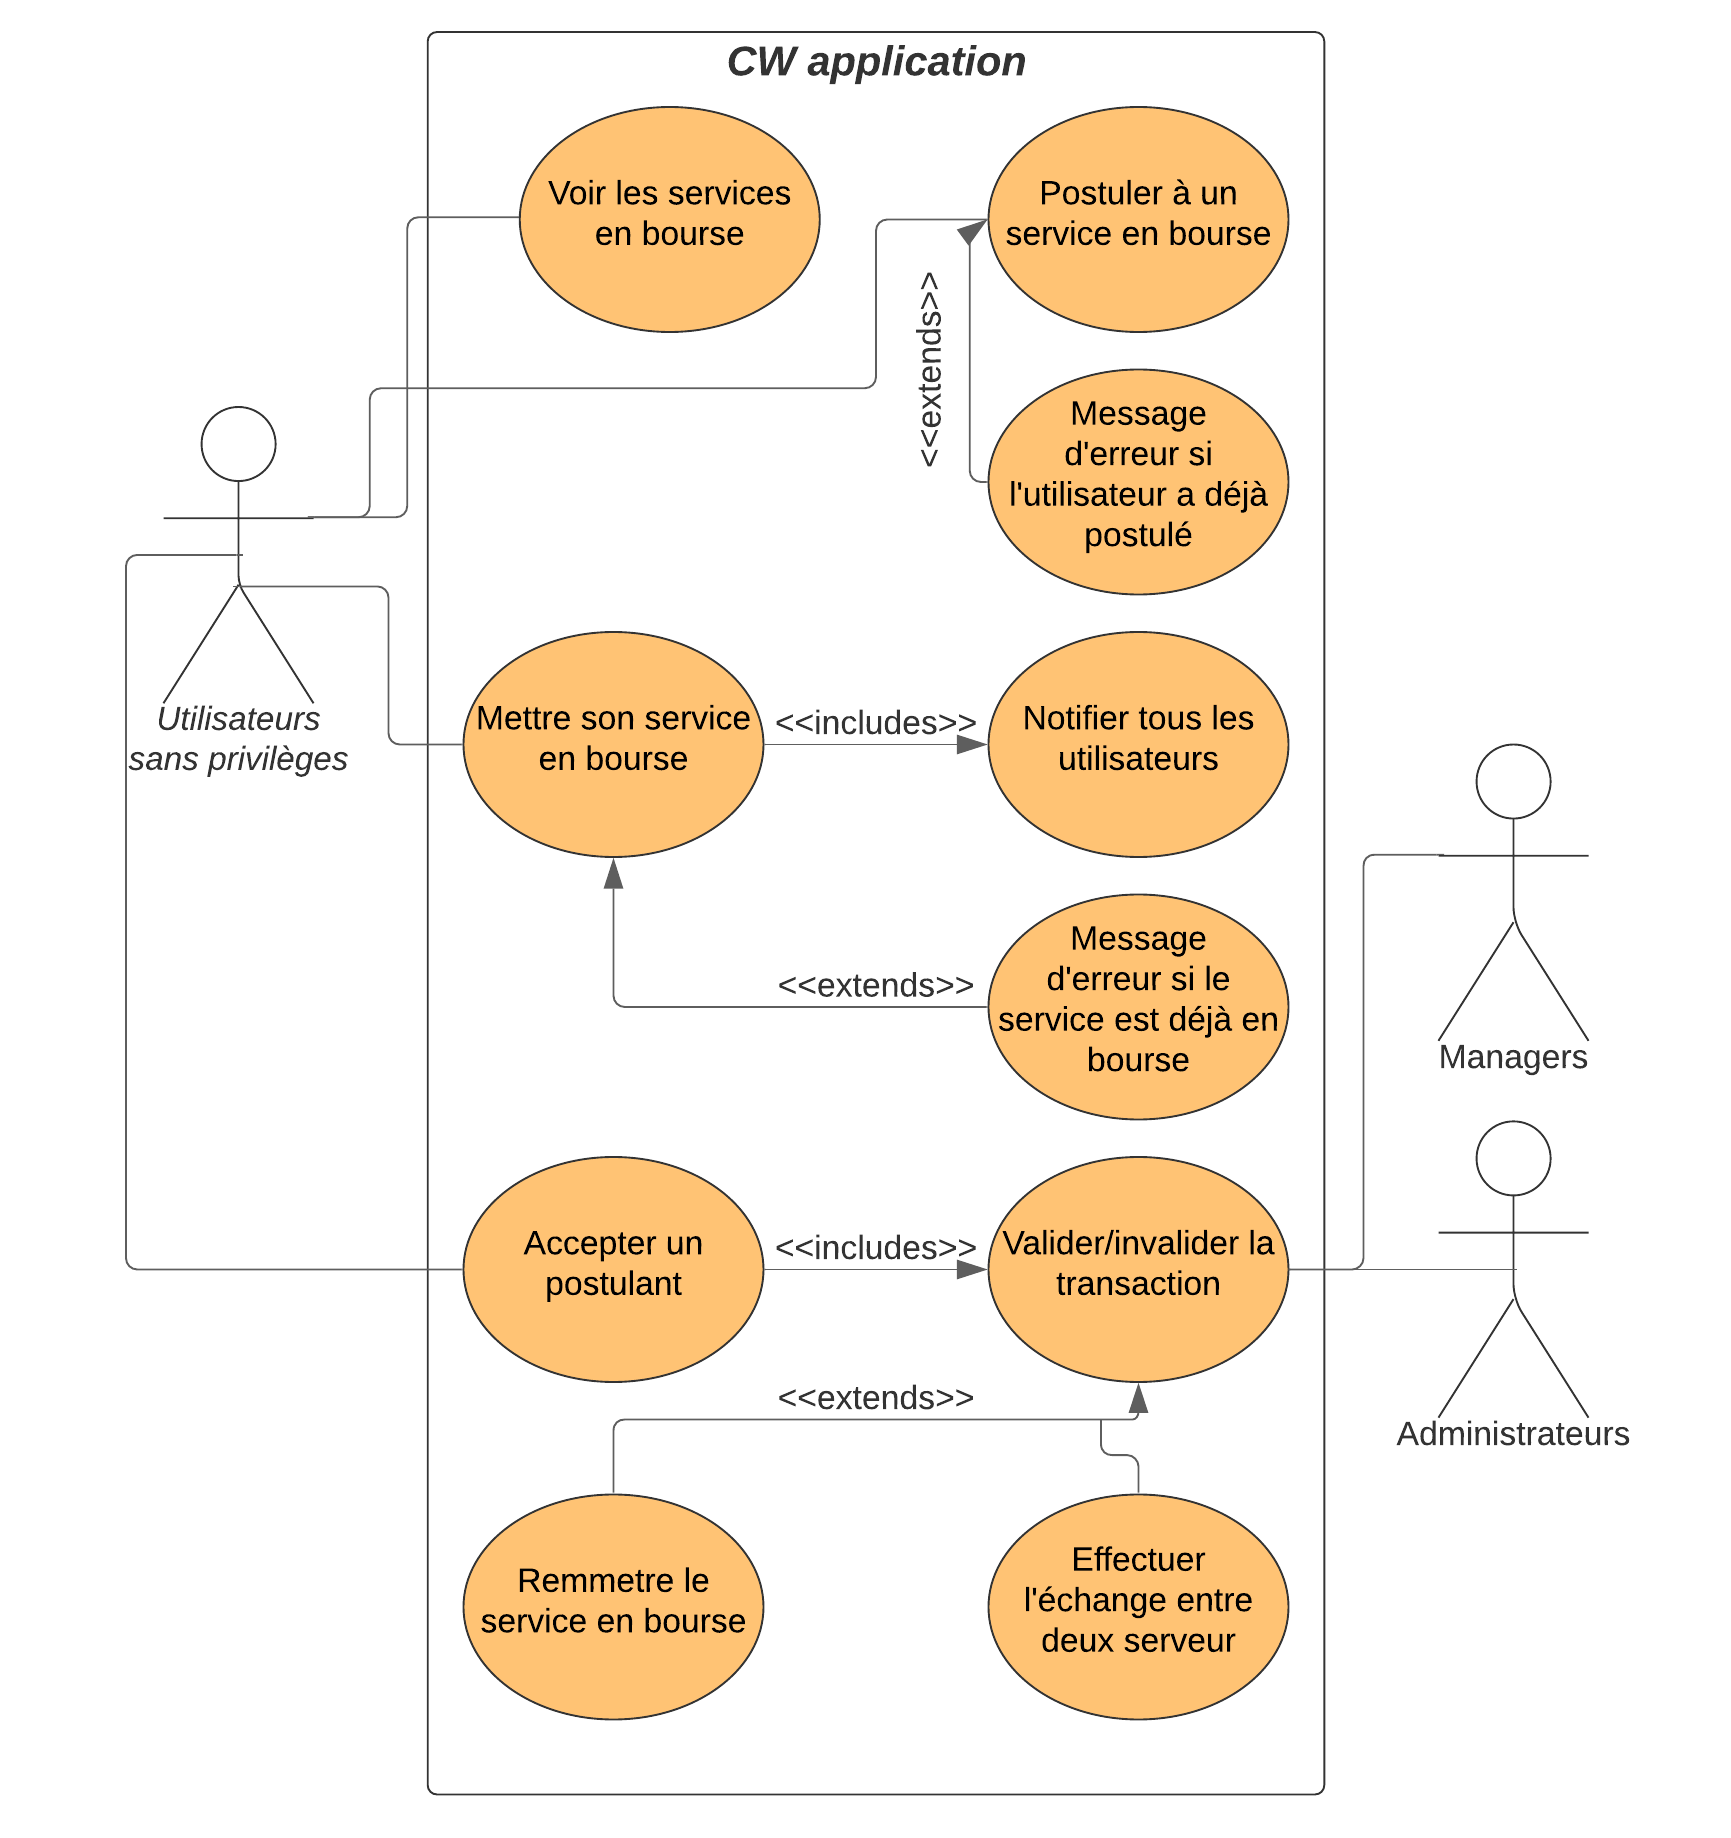
\includegraphics[width= 0.8\textwidth]{uses cases/BourseUC.png}
    \end{center}
    \caption{use case: mise en bourse des services}
\end{figure}

Dans un premier temps, tout utilisateur (normal, manager ou admin) doit pouvoir visualiser les services en bourse.
De plus, tout utilisateur doit pouvoir mettre son et uniquement son service en bourse. Ce qui engendre une notification à l'ensemble des utilisateurs de la disponibilité d'un nouveau service. 

Tout utilisateur doit pouvoir postuler à un service. Cela même si le postulant et celui l'ayant mis en bourse sont la même personne.

Seul l'utilisateur, quel qu'il soit, ayant mis le service en bourse, peut accepter un postulant. Ceci fait, seul un manager ou un administrateur doit valider ou invalider la transaction. Si l'utilisateur ayant mis le service en bourse a des privilèges il peut s'auto-valider la transaction.

Afin de simplifier le diagramme, les restrictions d'un utilisateur normal ont été mise en exergue.

\subsection*{Demande de renfort}

Pouvoir demander du renfort - des serveurs au doublage ou encore des doubleur - est la deuxième fonctionnalité \textit{must be}. 
\begin{figure}[!h]
    \begin{center}
        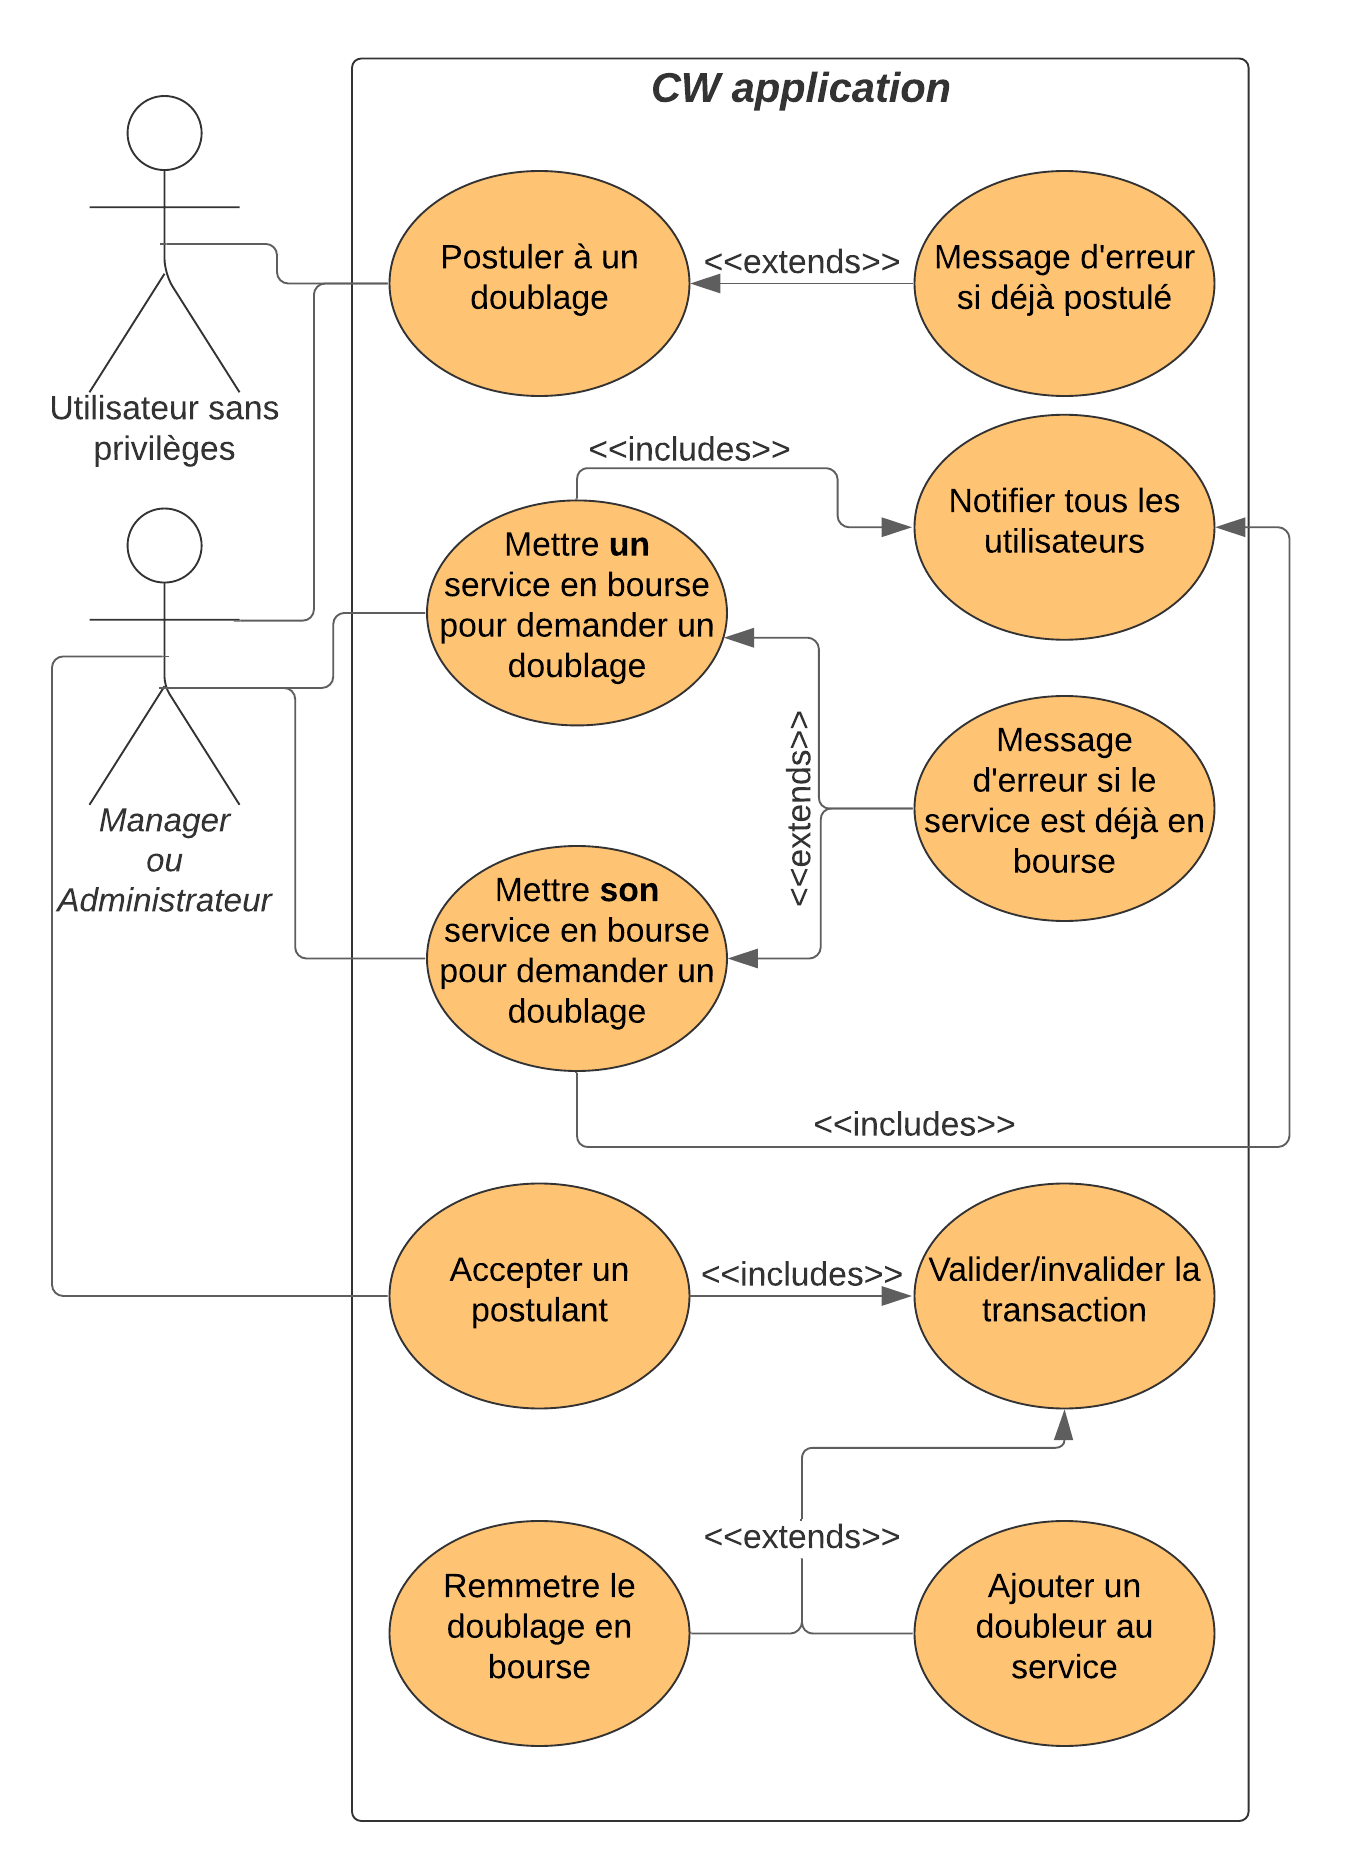
\includegraphics[width= 0.75\textwidth]{uses cases/doublageUC.png}
    \end{center}
    \caption{use case: mise en bourse d'un doublage}
\end{figure}

Les serveur$\cdot$euses sans privilèges ne peuvent que postuler pour des doublages déjà en bourse. Par contre, les utilisateurs avec privilèges peuvent compte à eux faire des demandes de doublage autant pour des services dans lesquels ils ne travaillent pas comme des services dans lesquels ils travaillent. Ils ont aussi la faculté d'accepter des postulants.

\section{Choix des technologies}
Le développement d'applications
pour smartphones est, depuis un peu plus d'une décennie, en pleine effervescence. Il existe, par
conséquent, une multitude de frameworks, services, langages, méthodologies et paradigmes liés à leur
développement.

Ces technologies aux noms exotiques, aux logos plus brillants les uns que les autres et aux
conférences accrocheuses qui leur sont dédiées, font que leurs différences relèvent plus
d'une stratégie marketing visant les informaticiens, réussie que des attributs
intrinsèques de la technologie en question.

Les fonctionnalités de l'application vues précédemment étant d'une complexité modérée et ne demandant pas de ressources importantes
comme tel pourrait être le cas pour une messagerie instantanée à grand échelle ou une application
utilisant abondamment un domaine spécifique de connaissance comme le \textit{machine learning}, le traitement d'images, les jeux vidéo, etc.
Exclu \textit{de facto} le choix d'une technologie basée exclusivement sur les performances ou sur le développement natif.

N'ayant jamais fait cela auparavant, il n'y a aucune préférence de ma part pour telle ou telle technologie.

Ces constats donnent lieu aux critères de sélection suivants:
\smallskip
\begin{itemize}
    \item Développement cross-plateforme
    \item Simplicité
    \item Apprentissage d'un langage plutôt qu'une multitude
    \item Vaste documentation et ressources d'apprentissage
\end{itemize}
\smallskip
Le premier critère est celui qui réduit le plus la liste des possibilités. En effet, les frameworks
permettant le développement d'applications pour Android et IOS ne se comptent pas en grand nombre. Il existe\footnote{Liste non exhaustive}:
\smallskip
\begin{itemize}
    \item Xamarin - Microsoft
    \item React Native - Facebook
    \item Flutter - Google
    \item Adobe PhoneGap - Adobe
    \item Ionic - MIT
\end{itemize}
\smallskip
Le choix parmi ces possibilités découle essentiellement de l'arbitraire. Toutefois, Ionic a été exclu car il est nécessaire de maîtriser HTML5 et par conséquent CSS mais encore Angular JS. Ce qui contredit le 3ème critère.

React native et Xamarin ont été exclus pour des raisons similaires. I.e. l'apprentissage de divers langages.

Finalement, à la suite d’un cours de Academind d'une durée de 40 heures portant sur les aspects les plus basiques du développement jusqu'au déploiement de l'application en passant par le routage, la gestion de requêtes http, la connexion à tout un écosystème de bases de données, l'utilisation de caméra et géolocalisation, et même sur comment changer le logo de l'application, le choix s'est porté sur Flutter.

Flutter est un framework crée par Google. Ce dernier offre, pour les applications, le service Firebase qui englobe :

\smallskip
\begin{itemize}
    \item Cloud Firestore
    \item Real time database
    \item Functions
    \item Machine learning
    \item Cloud messaging
    \item \dots
\end{itemize}
\smallskip
Firebase s'intègre, par conception, particulièrement bien et facilement à Flutter. Même s'ils sont
indépendants, leurs utilisation conjointe forme un seul écosystème plus facile à appréhender. Ainsi pour la
base de données, le choix a été la Real Time Database. Car cette dernière fournit une API REST.

De plus, toujours dans cet écosystème, \textit{Cloud messaging} est utilisé pour l'envoi des notifications et \textit{Functions} pour
effectuer des actions côté serveur lorsque la base de données subit des modifications.

\chapter[L'application]{Présentation de l'application}

Dans ce chapitre on présente l'application Crazy wolf. 
Au traver d'images commentées nous allons décrire plusieurs scénarios
d'utilisation.
\section[Authentification \& écran d'accueil - Scénario I]{Scénario I}
\subsection*{Authentification \& écran d'accueil}
Ici la serveuse Kim, qui n'a pas de privilèges, c'est-à-dire qu'elle n'est 
ni manager ni administratice, se connecte et accède au premier écran possible.
Puis elle, click sur "Mes services".

\begin{figure}[!h]
    \centering
    \begin{subfigure}{.3\textwidth}
        \centering
        
\includegraphics[width=0.9\linewidth]{screenshots/scenario_01/login.png}
        \caption{login}
        \label{fig:login}
    \end{subfigure}
    \begin{subfigure}{.3\textwidth}
        \centering
        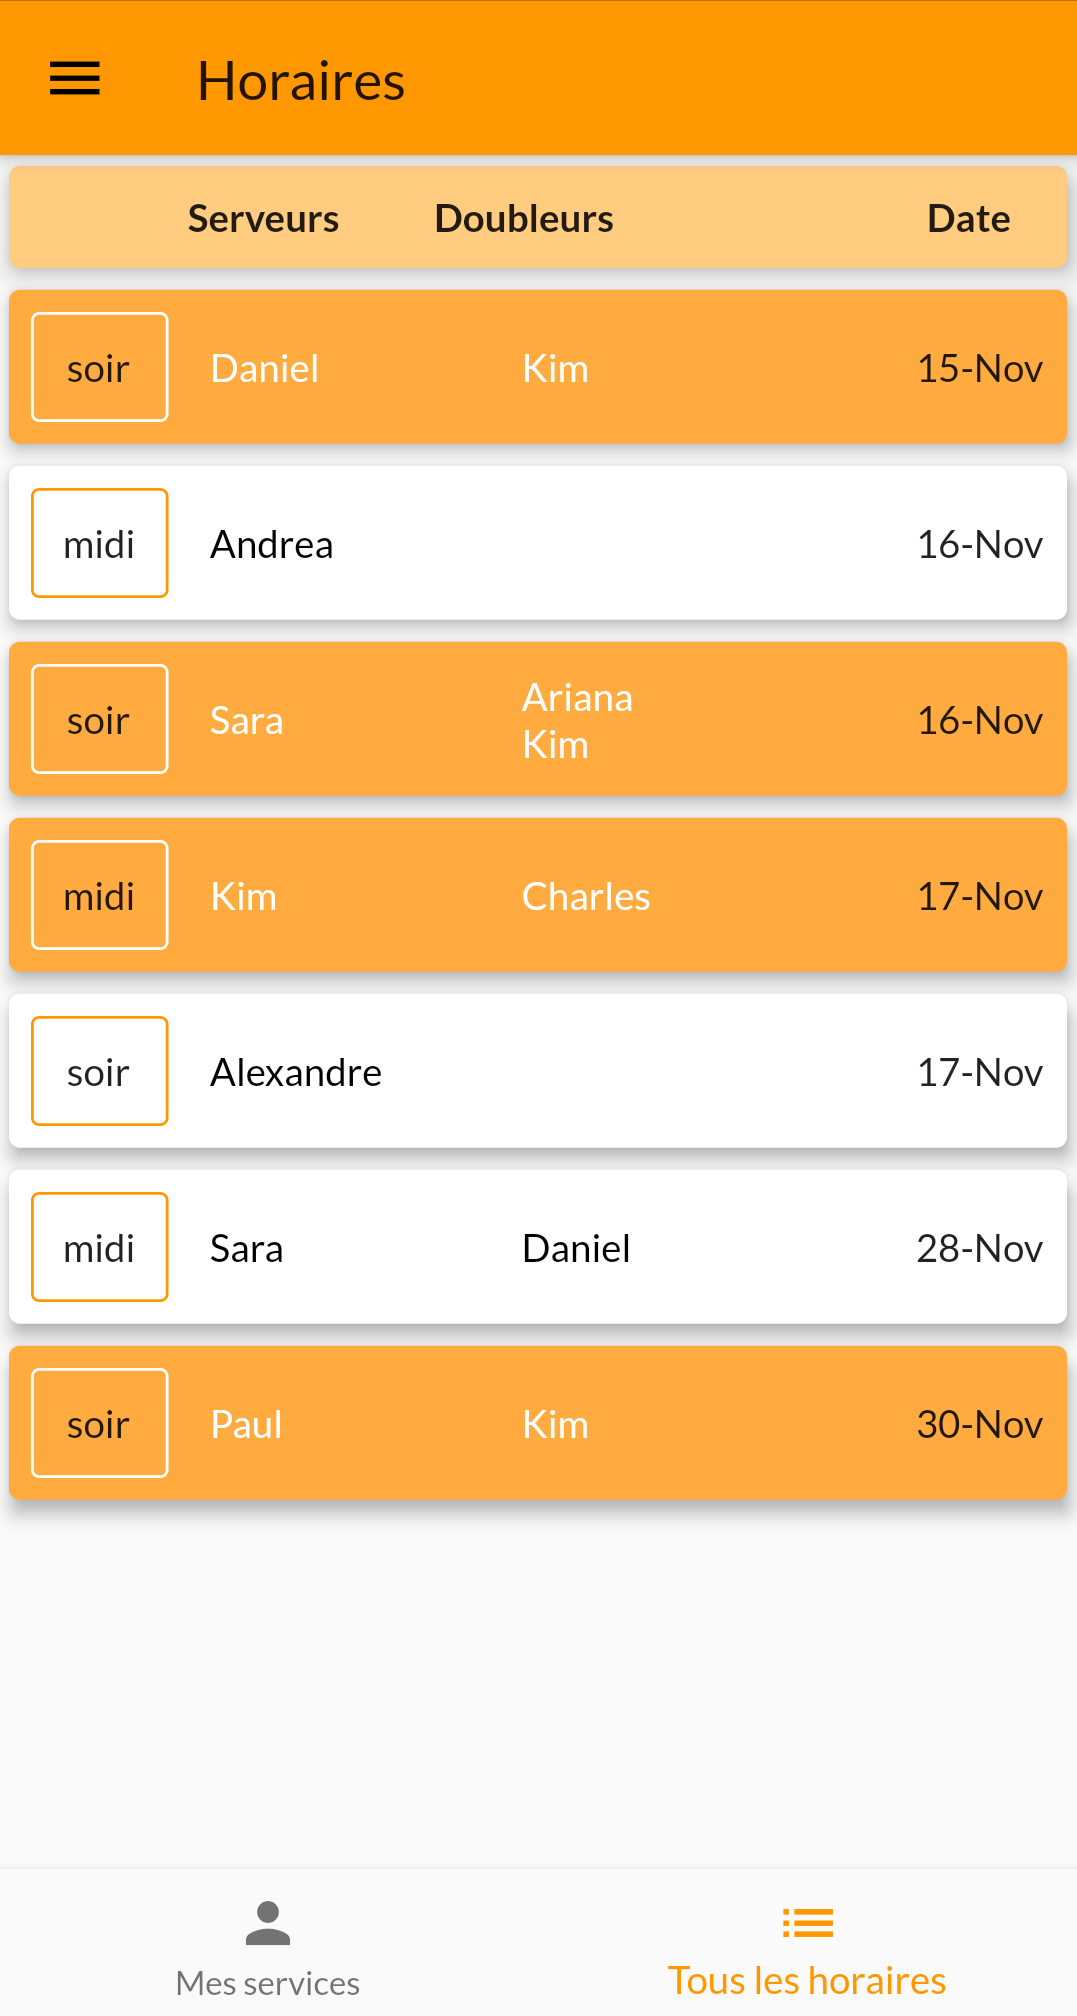
\includegraphics[width=0.9\linewidth]{screenshots/scenario_01/horaires.png}
        \caption{horaires}
        \label{fig:horaires}
    \end{subfigure}
    \begin{subfigure}{.3\textwidth}
        \centering
        
\includegraphics[width=0.9\linewidth]{screenshots/scenario_01/mesHoraires.png}
        \caption{mes horaires}
        \label{fig:mesHoraires}
    \end{subfigure}
    \caption{scénario I}
    \label{fig:scen01}
\end{figure}

L'utilisateur doit dans un premier temps se connecter à l'aide d'identifiants déjà existant dans l'écran \ref{fig:login}. Une fois l'addresse mail et le mot de passe saisis, 
l'écran \ref{fig:horaires} s'affiche. 


On y voit l'ensemble des horaires de travail. Les services sont définis par
\begin{itemize}
    \item le type: midi ou soir.
    \item un ou plusieurs serveurs.
    \item zero, un ou plusieurs doubleurs.
    \item la date
\end{itemize}
Les services sont ordonnés par date, les jours précédents au moment de la connection ne 
sont pas affichés. Les horaires correspondant à la personne authentifié sont de couleurs orange.

Les services sont affichés sous forme de liste scrollable.

On peut également naviguer à l'aide du menu inférieur à "mes services" où seuls les horaires du serveur authentifié sont affichés. Comme on le voit 
dans \ref{fig:mesHoraires}

\section[Mise en bourse d'un service - Scénario II]{Scénario II}
    \subsection*{Mise en bourse d'un service}
    Supposons que Kim, la serveuse authentifiée ne puisse pas travailler le 17 novembre.
    Elle souhaite donc se faire remplacer. Pour se faire, dans l'onglet 
    "horaires", elle peut mettre son service en bourse en glissant le 
    service en question sur la gauche.
    \begin{figure}[!h]
        \centering
        \begin{subfigure}{.45\textwidth}
            \centering
            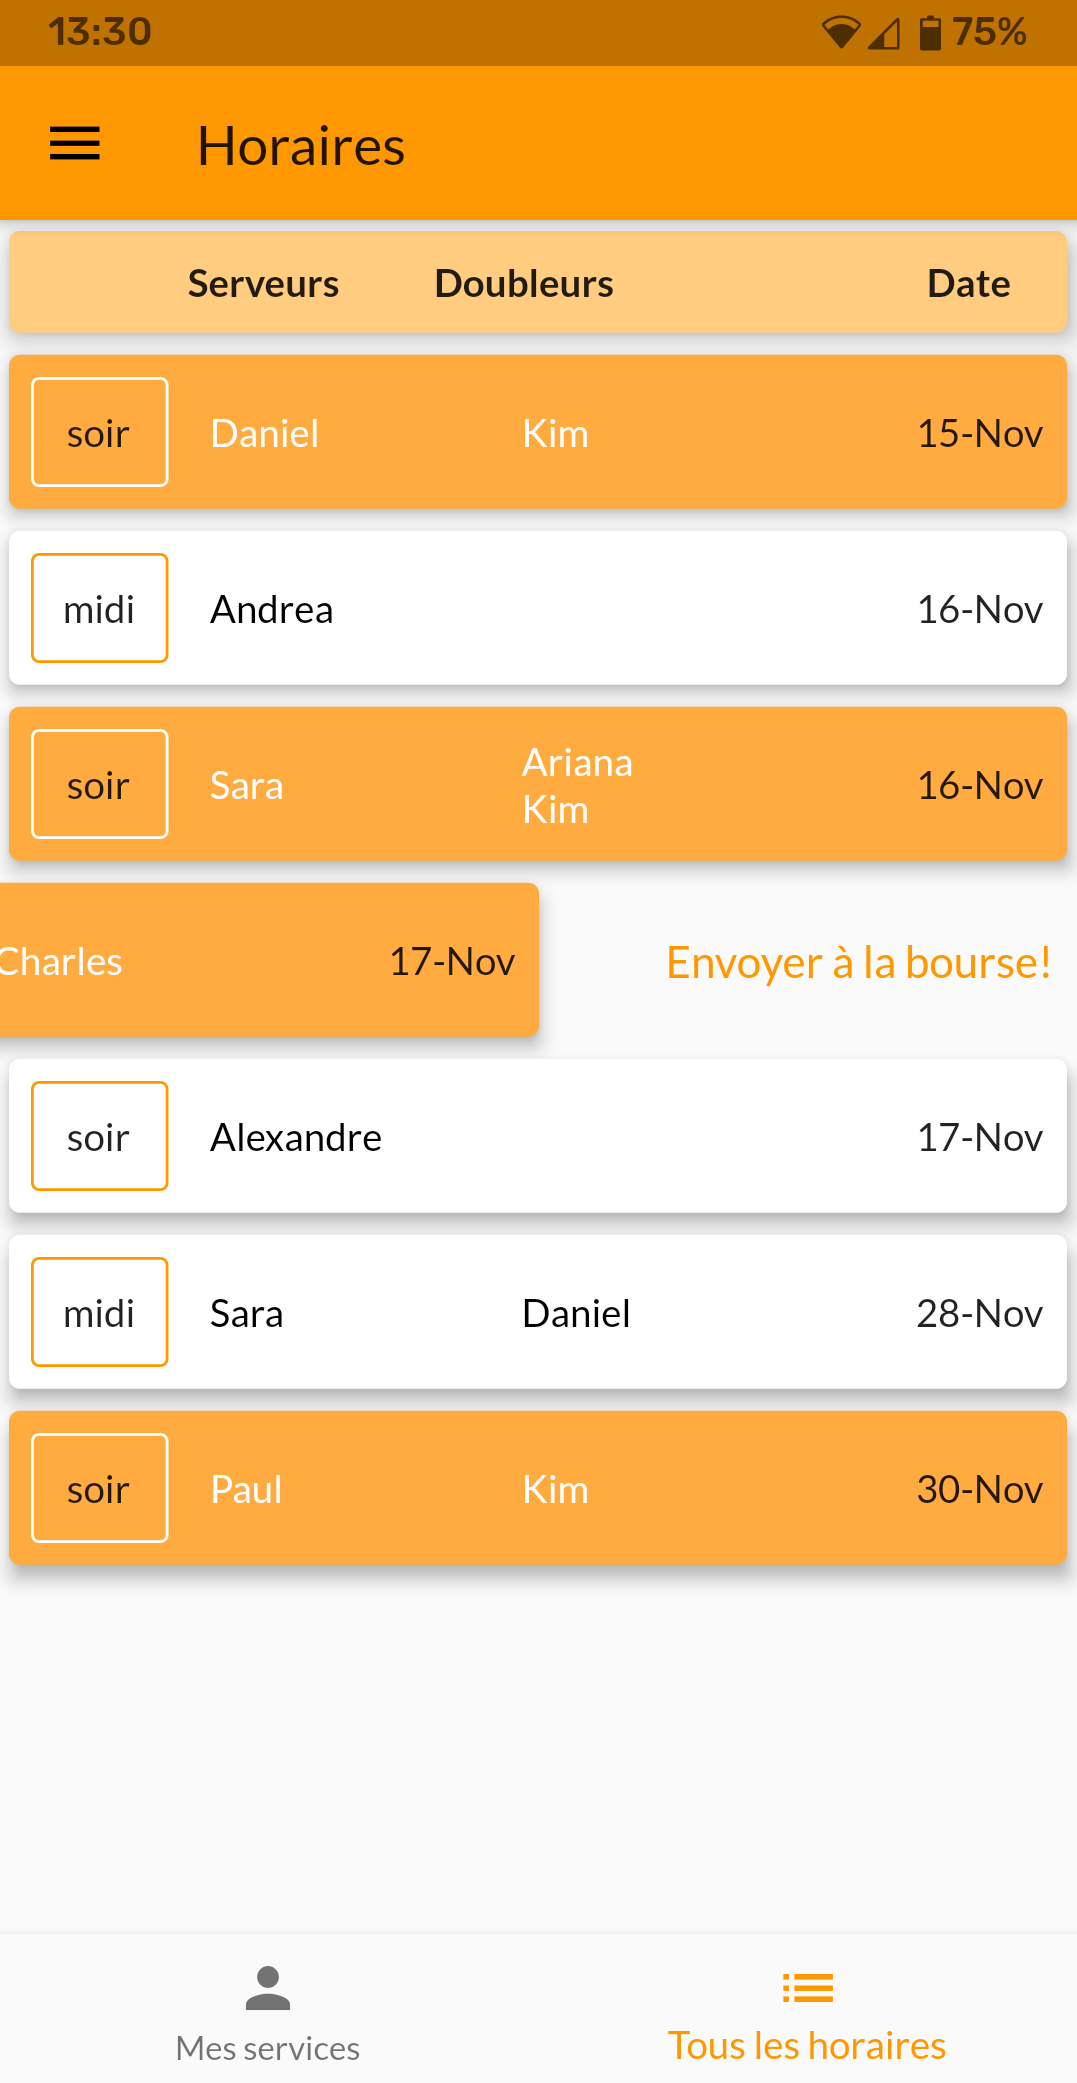
\includegraphics[width=0.6\linewidth]{screenshots/scenario_02/mise_en_bourse.png}
            \caption{mise en bourse}
            \label{fig:mise_en_bourse}
        \end{subfigure}
        \begin{subfigure}{.45\textwidth}
            \centering
            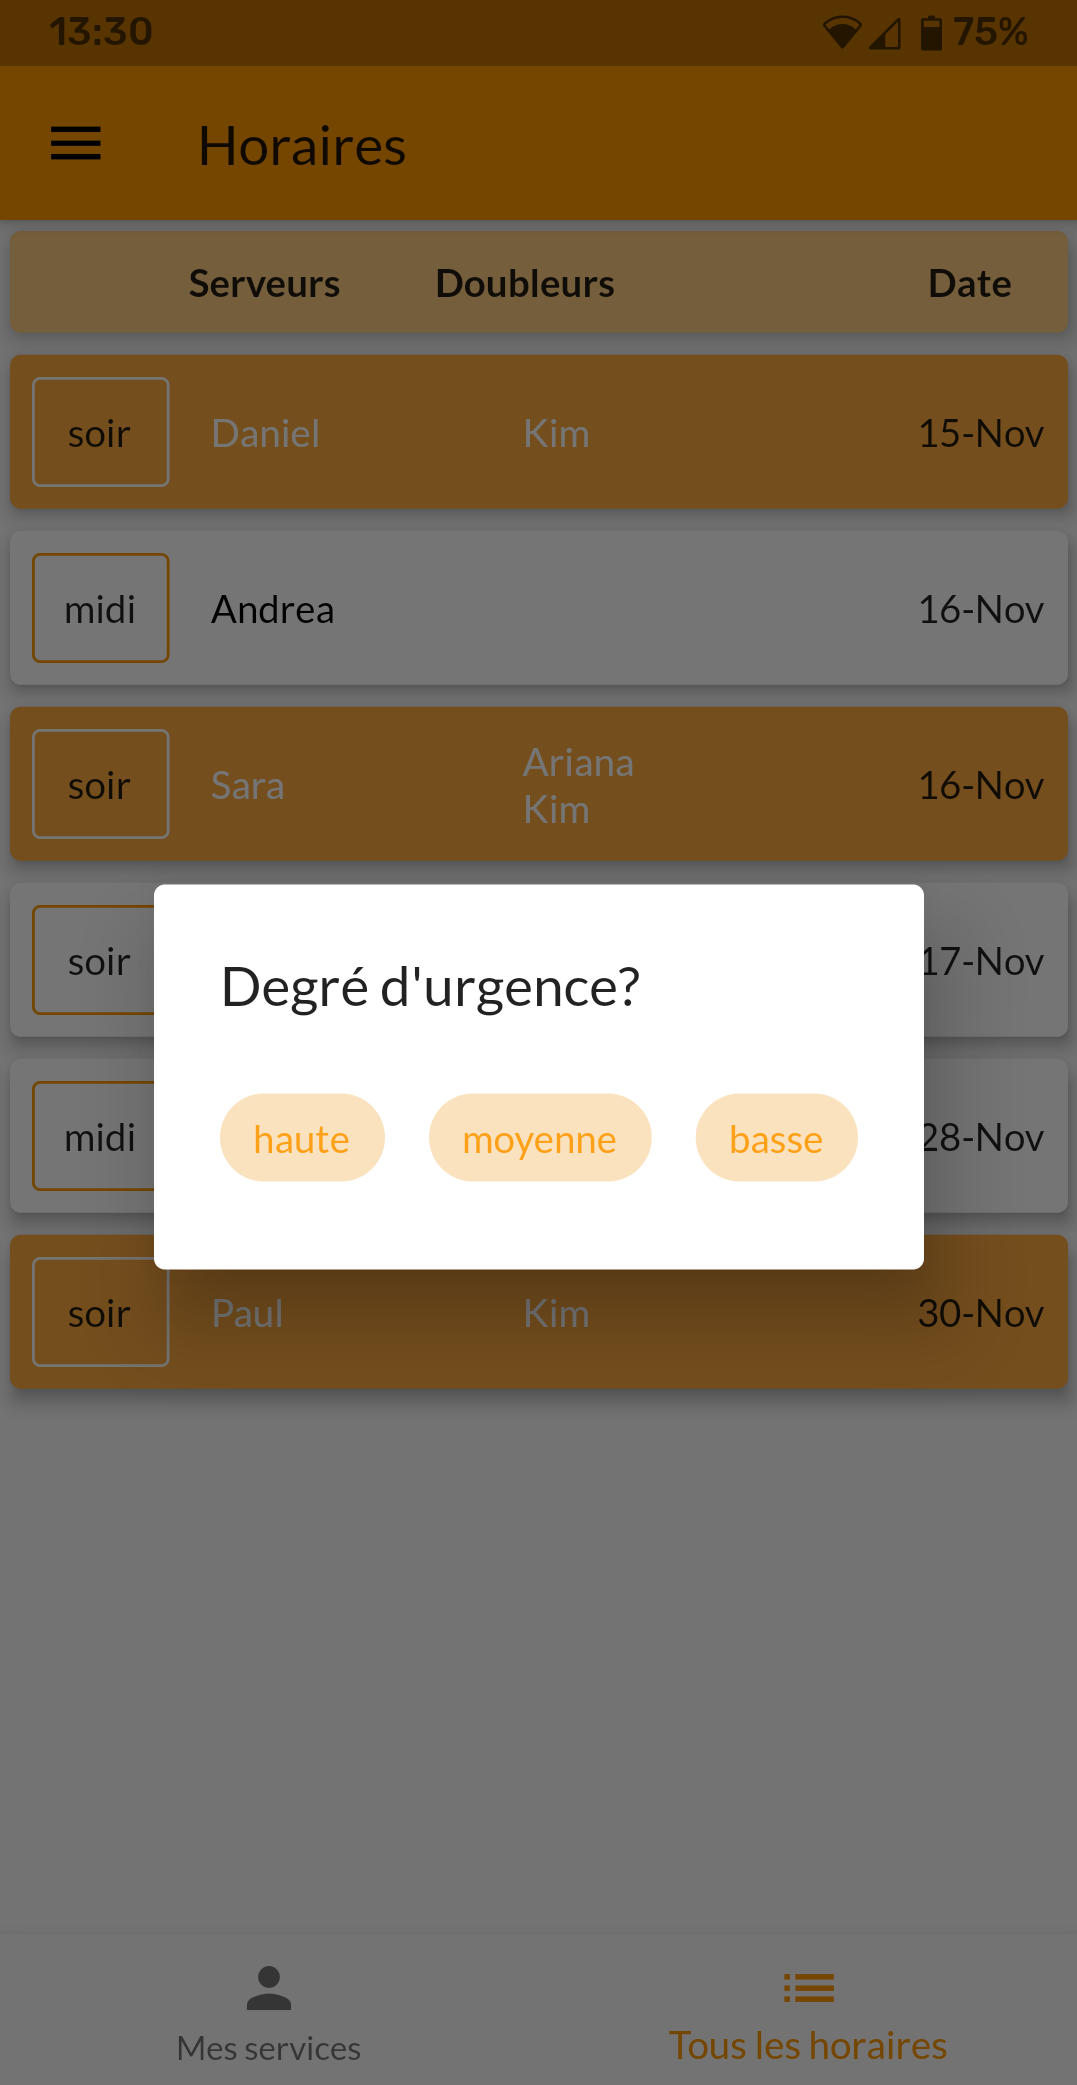
\includegraphics[width=0.6\linewidth]{screenshots/scenario_02/urgence.png}
            \caption{urgence}
            \label{fig:urgence}
        \end{subfigure}
        \caption{scénario II - a}
        \label{fig:scen02a}
    \end{figure}

Une fois le glissement éffectué un popup est s'affiche \ref{fig:urgence} demandant
à quel point le remplacement est urgent. Une fois que l'utilisateur à répondu, le service est mis
en bourse. Un snakbar s'affiche pour le notifier que l'action à réussi.

Si l'action est réussie, tous les utilisateur de l'application sont notifié \ref{fig:notif} comme quoi un 
nouveau service est disponible. La notification informe sur la disponibilité d'un service ainsi que 
l'urgence requise à y répondre. 

Suit à ça, l'utilisatrice peut naviguer à l'aide du menu lateral \ref{fig:menu_sans_droits} où s'affichent les options
de navigation suivante: 
\begin{itemize}
    \item Horaires: Pour aller à l'écran "Horaires" \ref{fig:horaires}
    \item Logout: Pour se déconnecter, qui revoit à l'écran \ref{fig:login}
    \item Bourse: Pour aller à l'écran bourse aux jobs \ref{fig:bourse}
\end{itemize}
\begin{figure}[!h]
    \begin{subfigure}[]{.3\textwidth}
        \centering
        
\includegraphics[width=0.9\linewidth]{screenshots/scenario_02/notification.png}
        \caption{notification}
        \label{fig:notif}
    \end{subfigure}
    \centering
    \begin{subfigure}{.3\textwidth}
        \centering
        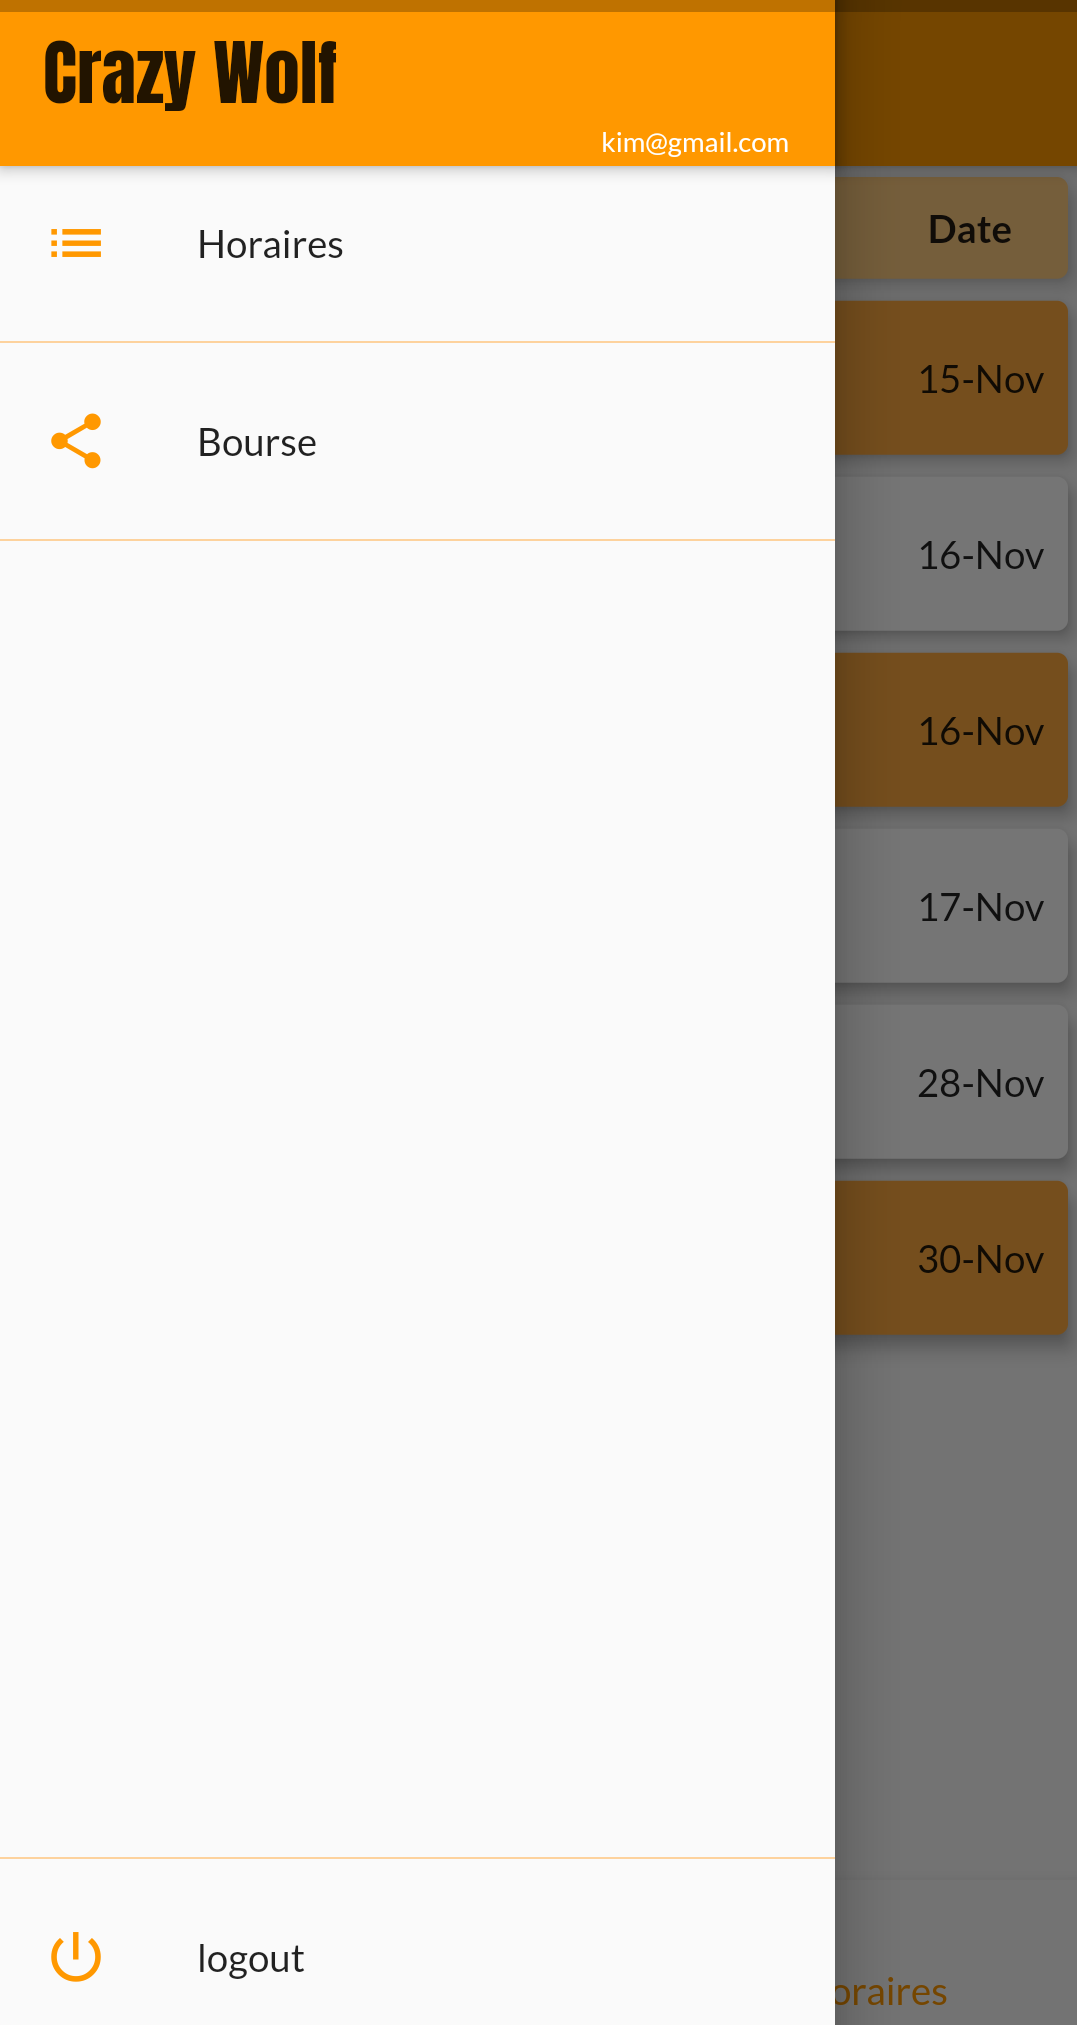
\includegraphics[width=0.9\linewidth]{screenshots/scenario_02/menu_serveur_normal.png}
        \caption{menu sans privilèges}
        \label{fig:menu_sans_droits}
    \end{subfigure}
    \begin{subfigure}{.3\textwidth}
        \centering
        
\includegraphics[width=0.9\linewidth]{screenshots/scenario_02/bourse_jobs.png}
        \caption{bourse}
        \label{fig:bourse}
    \end{subfigure}
    \caption{scénario II - b}
    \label{fig:scen02b}
\end{figure}

Dans l'onglet "Bourse aux jobs" son service est disponible à toute personne souhaitant y postuler. 
Cet onglet est partagé parmis tous les utilisateurs de l'application.

La couleur représente le degré d'urgence. Ainsi la convention suivante est appliqué:
\begin{itemize}
    \item rouge: implique une urgence élevée.
    \item jaune: implique une urgence moyenne.
    \item vert: implique une urgence basse.
\end{itemize}

L'onglet "Bourse aux jobs" affiche tous les service actuellement en bourse sous
forme de liste scrollable. L'utilisateur ayant mis son service en bourse
doit patienter à ce que quelqu'un y postule.

Les utilisateur sans privilèges sont authorisé à mettre un service en bourse uniquement s'ils y travaillent.

\section[Postuler pour un service - Scénario III]{Scénario III}
    \subsection*{Postuler pour un service}
    Dans la continuation du scénario précédent, après avoir été notifiés,
    deux serveurs vont postuler au nouveau service mis
    en bourse. Leurs parcours étant identiques, nous allons en montrer qu'un.
    Supposons qu'ils se soient authentifié comme vu en \ref{fig:login} et qu'ils se trouvent
    dans l'onglet "Bourse au jobs" \ref{fig:bourse}.

    \begin{figure}[h]
        \centering
        
\includegraphics[width=.3\linewidth]{screenshots/scenario_03/postuler.png}
        \caption{postuler}
        \label{fig:postuler}
    \end{figure}

    Alors, ils peuveunt glisser le service auquel ils souhaitent postuler sur
    la gauche. À nouveau, si l'opération réussi, un snackbar apparaît pour l'indiquer.

    L'utilisateur ayant mis le service en bourse doit procéder à l'acceptation
    d'un seul postulant. Dans "Bourse aux jobs" \ref{fig:bourse} les éléments de 
    la liste sont clickable. Lorsqu'un utilisateur click deux options sont possibles:

    \begin{figure}[!h]
        \centering
        \begin{subfigure}{.45\textwidth}
            \centering
            
\includegraphics[width=0.6\linewidth]{screenshots/scenario_03/detail_auth.png}
            \caption{ayant mis le service en bourse}
            \label{fig:detail_auth}
        \end{subfigure}
        \begin{subfigure}{.45\textwidth}
            \centering
            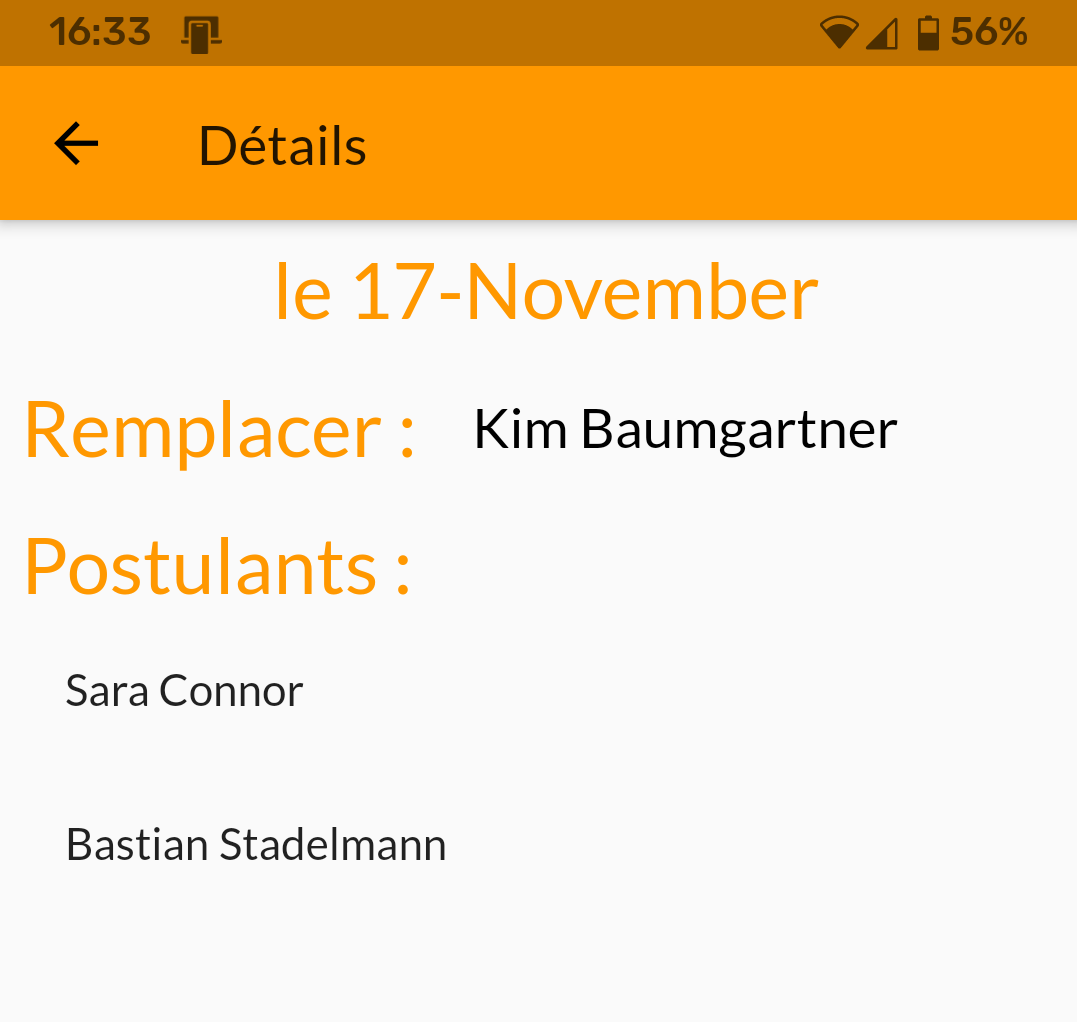
\includegraphics[width=0.6\linewidth]{screenshots/scenario_03/detail_non_auth.png}
            \caption{autre}
            \label{fig:detail_non_auth}
        \end{subfigure}
        \caption{scénario III}
        \label{fig:scen03}
    \end{figure}

    S'il s'agit de l'utilisateur ayant mis le service en bourse à l'occurence Kim, l'écran détails tel que \ref{fig:detail_auth} s'affiche.
    S'il s'agit de n'importe quel autre utilisateur alors l'écran détails s'affiche comme dans \ref{fig:detail_non_auth}

    Ainsi, seul l'utilisateur ayant mis le service en bourse est en mesure d'accpter un ou une remplaçante. Pour se faire,
    Kim doit appuyer sur le bouton accepter de la personne de son choix.

\section[Valider un échange - Scénario IV]{Scénario IV}
    \subsection*{Valider un échange}
    Toujours dans la continuation de notre exemple, nous allons voir ici 
    la validation d'un échange. En effet, même si un utilisateur
    à accepté un remplaçant pour son service. Il faut encore que cette
    transaction soit validée par un utilisateur avec privilèges.

    Il existe trois types d'utilisateurs:
    \begin{center}
        \begin{tikzpicture}
            \node[] at (0.5,2) {normal};
            \draw[color=RoyalRed] (2,2) circle (3.5cm);
            \node[] at (2.5,1.5) {manager};
            \draw[color=RoyalRed] (1,2) circle (2.5cm);
            \node[] at (4.5,1.0) {admin};
            \draw[color=RoyalRed] (0,2) circle (1.5cm);
        \end{tikzpicture}
    \end{center}
    


\chapter[Programmation]{Elements de programmation}

    \section{Choix des téchnologies}

    \section{La base de données}
        \subsection{La méthodologie REST}
        \subsection{REST appliqué à Dart}

    \section{Flutter}
        \subsection{Les widgets}
        \subsection{Flux des données}
            \subsubsection{Par constructeur}
            \subsubsection{Provider \& Consumer}
            
    \section{Notifications}
    
    \section{Sécurité}
        \subsection{Authentification}
        \subsection{Firebase rules}

\chapter[Le client]{Coordination avec le client}
    \section{Introduction}
    \section{Echanges}
    \section{Problèmes}

    

\chapter{Conclusion}
\blindtext
\blindtext


\end{document}